%%Introduction

In this Section, we consider models with a photon, a W boson, a Z boson or a Higgs boson in the final state, 
accompanied by Dark Matter particles that either couple directly to the boson or are mediated by 
a new particle. The experimental signature is identified as \textit{V+MET}. 

These models are interesting both as extensions of models where the gluon provides 
the experimentally detectable signature, 
and as stand-alone models with final states that cannot be generated by the models in
Section~\ref{subsec:MonojetLikeModels}.

%%%Classification of models

%FIXME: CD - the tufte.cls on SVN does not like citep. Why? Will look into it later.
\begin{figure}[h!]
  \centering
    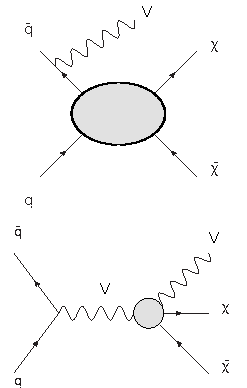
\includegraphics[width=0.5\textwidth]{figures/VPlusMET_EFT}
  \caption{Sketch of EFT models for V+MET searches, adapted from~\citep{Nelson:2013pqa}. \label{fig:VPlusMET_EFT}}
\end{figure}
% 
The models considered can be divided in four categories:
\begin{description}
 \item[EFT models where the boson is radiated from the initial state] As depicted in 
 the top diagram of Figure~\ref{fig:VPlusMET_EFT}, these  models follow the nomenclature and theory 
 for the EFT benchmarks commonly used by MET+X searches~\cite{Goodman:2010ku}. 
 \item[EFT models where the boson is directly coupled to DM] Shown in the bottom of Figure~\ref{fig:VPlusMET_EFT},
 these models allow for an EFT vertex that directly couples the boson to Dark Matter. 
 \item[Simplified models where the boson is radiated from the initial state] These models follow those
 already described in Section~\ref{subsec:MonojetLikeModels}, replacing the initial state gluon with a boson.
 \item[V-specific simplified models] These models postulate direct couplings of new mediators
 to bosons, e.g. they couple the Higgs boson to a new scalar~\cite{Carpenter:2013xra}. 
\end{description}

The following Sections describe the models within these categories, 
the parameters for each of the benchmark models chosen,
the studies towards the choices of the parameters to be scanned, 
and finally point to the location of their Matrix Element 
implementation. 

\paragraph{EFT models with ISR boson radiation}

Searches in the mono-jet final state are generally more sensitive with respect to final
states including bosons, due to the much larger rates of jet+MET signal events with 
respect to radiation of bosons~\cite{Zhou:2013fla}.
The rates for the H+MET signature in these models are too low for EFT models 
to be considered a viable benchmark~\cite{Carpenter:2013xra}.
However, the presence of photons~\cite{Khachatryan:2014rwa, Aad:2014vka}, 
leptons from W and Z decays~\cite{Khachatryan:2014tva, Aad:2014vka, ATLAS:2014wra} 
and W or Z bosons decaying hadronically~\cite{Aad:2013oja}
allow to reject the background more effectively, making Z/gamma/W+MET search results for 
simple EFT benchmarks still worth comparing with jet+MET.
Furthermore, in the case of W boson radiation, the values of the 
couplings to up- and down-type quarks determine the interference between
the radiation of a W from the up or from the down quark~\cite{Bai:2012xg}. 
In case of constructive interference, the W+MET signature is more sensitive
than the jet+MET signature (insensitive to the values of couplings). 
%The couplings to up and down quark are defined as $C(u)$ and $C(d)$ 

\paragraph{EFT models with direct DM-boson couplings}

A complete list of effective operators with direct DM/boson couplings, 
up to dimension 7, can be found in~\cite{Cotta:2012nj}.

\paragraph{Simplified models with ISR boson radiation}

\paragraph{Specific simplified models}
